\documentclass[a4paper]{scrreprt}

\usepackage{scrhack}
\usepackage{graphicx}
\usepackage[utf8]{inputenc}

\addtokomafont{titlehead}{\flushright}
\addtokomafont{subject}{\vspace{3cm}\flushleft}
\addtokomafont{title}{\flushleft}
\addtokomafont{subtitle}{\flushleft}
\addtokomafont{author}{\flushleft\setlength{\tabcolsep}{0pt}}
\addtokomafont{date}{\flushleft}
\addtokomafont{publishers}{\flushleft}

\titlehead{
\includegraphics[scale=2]{../templates/logo_en}}
\subject{Software Engineering and Design}
\title{Software Architecture}
\subtitle{Mental Health Care Patient Management System (MHC-PMS)}
\author{
\begin{tabular}{l}
\normalfont\bfseries{Team White:}\\
Dellsperger Jan\\
Ellenberger Roger\\
Sheppard David\\
Sidler Matthias\\
Spring Mathias\\
Thöni Stefan
\end{tabular}
}
\date{\today}
\publishers{Version 1.0}

\begin{document}

\begin{titlepage}
	\maketitle
\end{titlepage}



\chapter{Übersicht}

\section{Systemrequirements}
Dieser Abschnitt beschreibt, welche Requirements im Projekt umgesetzt werden und wie die Umsetzung aussieht (siehe Dokument Requirements-Specification aus Task 4). Wir konzentrieren uns auf die Functional Requirements.

\subsection{Darstellung Dashboard}
Die Darstellung des Dashboards wird im Presentation Layer realisiert.

\subsection{Konfiguration Dashboard}
Der veränderbare Teil der Daten beschränkt sich auf die benutzerspezifischen Konfigurationen des Dashboards. Damit die \textbf{Datenpersistenz} gewährleistet wird, wird ein Container benötigt, welcher diese Daten abspeichert. Die Benutzerkonfiguration legen wir daher in einer Datenbank ab. Es ist angedacht, die Datenbank auf dem gleichen Server zu betreiben, der auch die Datenquelle fürs Reporting enthält.

\subsection{Reporting anzeigen}
Die Anzeige der Reports wird im Presentation Layer realisiert.

\subsection{Schnittstelle DBS} 
Die Daten, welche fürs Reporting verwendet werden, sind nicht in Verantwortung der Applikation und es wird bloss lesend darauf zugegriffen. Die Anbindung wird im Data Access Layer umgesetzt.

\subsection{Kennzahlen}
Die Quelldaten fürs die Berechnung der Kennzahlen, werden aus einer externen Datenquelle geholt (Siehe Schnittstelle DBS).






\chapter{Architektur}
\paragraph{Layering Pattern}
Für die Gesamtarchitektur verwenden wir das Layering Pattern. Die Applikation wird aufgeteilt in die Layer \textit{Presentation}, \textit{Business Logic} und \textit{Data Access}. Zudem existiert der Layer \textit{Model}. Dieser zieht sich über alle Layers hinweg und enthält die Model-Logik aus dem MVC-Pattern.


\paragraph{MVC Pattern}
Die Grundstruktur des MVC-Pattern wird durch Vaadin implementiert. Die Klassen von Model, View und Controller werden für diese Applikation erstellt. Vaadin gibt hierzu aber die Vorgaben, wie das gemacht werden muss.


\paragraph{Client Server Pattern}
Die Applikation basiert zudem auf dem Client-Server Pattern. Clientseitige Zugriff geschieht via Web-Browser. Die dazu benötigte Logik stellt das Framework Vaadin bereit.

\bigskip

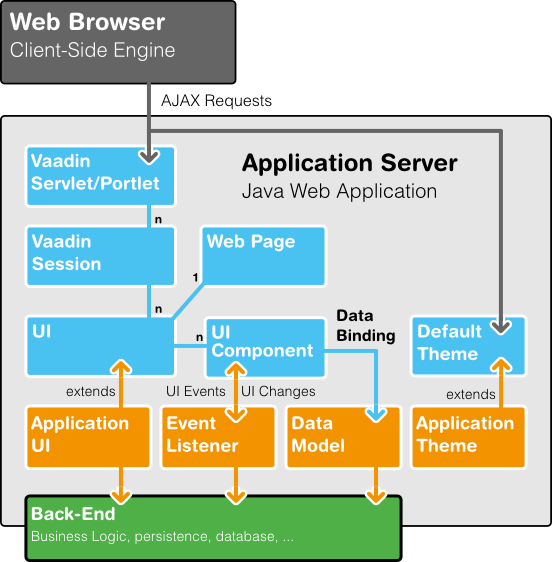
\includegraphics[width=0.7\textwidth]{img/vaadin-arch.png}


\section{Presentation Layer}
Für die Bereitstellung der grafische Oberfläche nutzen wir Vaadin. 



\section{Business Logic Layer}



\section{Data Access Layer}
Dieser Layer realisiert die Anbindung an das Datenbank-Backend. Wir verwenden JDBC um die Verbindung auf das Datenbanksystem (DBS) herzustellen. Als DBS verwenden wir einen MySQL-Server (bzw. den kompatiblen MariaDB-Server).




\section{Model Layer}








\end{document}